\chapter{坐标轴}

\section{各种距离}

\subsection{切比雪夫距离}

\begin{definition}[切比雪夫距离（Chebyshev）] \label{def:int} 
\[
d(P, Q) = \max(|x_1 - x_2|, |y_1 - y_2|)
\]

理解：横坐标差和纵坐标差，哪个大，距离就是哪个。就像走棋盘，横竖都能走，但步数由差得多的方向决定。

\subsection*{做法}
\begin{itemize}
    \item \textbf{求距离}：计算横坐标差、纵坐标差，取较大的数。
    \item \textbf{反求坐标}：设未知数，分情况（哪个差更大）列绝对值方程。
    \item \textbf{最值问题}：想让最大值变小，就让横差和纵差尽量接近；想让最大值变大，就只拉大其中一个差。
\end{itemize}

\subsection*{注意}

\begin{itemize}
    \item 切比雪夫距离相等的点，不在通常的垂直平分线上，而是在一条斜着的线上。
    \item 不要用“勾股定理”的距离去猜，它俩不一样。
\end{itemize}

\end{definition}


\subsection{曼哈顿距离}

\begin{definition}[曼哈顿距离]
\[
d(P, Q) = |x_1 - x_2| + |y_1 - y_2|
\]

理解：只能横平竖直移动的总步数，如出租车在网格街道行驶。


\subsection*{做法}

\begin{itemize}
    \item \textbf{求距离}：直接相加。
    \item \textbf{已知距离画区域}：
    \[
    |x - a| + |y - b| = r
    \]
    是菱形（旋转45°正方形）。
    \item \textbf{最值}：横、纵坐标差的绝对值分别考虑再合并。
\end{itemize}

\subsection*{注意}

\begin{itemize}
    \item 曼哈顿“圆”是菱形，不是圆。
    \item 多点求和时分坐标处理更简单。
\end{itemize}

\end{definition}


\subsection{绝对值比较型}

\begin{definition}[绝对值比较型]
如
\[
k = \max(|x|, |y|)
\]
或
\[
k = \min(|x|, |y|)
\]

理解：单点自身横纵坐标绝对值比大小，取大或取小。

\end{definition}

\subsection*{做法}

\begin{itemize}
    \item \textbf{给点求值}：算 \(|x|, |y|\)，按要求取。
    \item \textbf{满足条件的点集}：
    \[
    \max(|x|, |y|) = 2
    \]
    是边长为4的正方形边界。
    \item \textbf{线段上恒成立}：用参数表示，代不等式组。
\end{itemize}

\subsection*{注意}

\begin{itemize}
    \item 分清取大还是取小，等号通常 \(|x| = |y|\)。
    \item 这是单点特征，不是两点间距离。
\end{itemize}


\section{西城期末第26题}


在平面直角坐标系中，对于点 \(P_1(x_1, y_1)\)、\(P_2(x_2, y_2)\)、\(\cdots\)、\(P_n(x_n, y_n)\)，给出如下定义：把 \(x_1 + y_1,\ x_1 + y_2,\ \cdots,\ x_n + y_n\) 这 \(n\) 个数中的最大值记为 \(d_{\text{max}}\)，最小值记为 \(d_{\text{min}}\)，将 \(d_{\text{max}} - d_{\text{min}}\) 称为点 \(P_1, P_2, \cdots, P_n\) 的“特征值”，记作 \(T[P_1, P_2, \cdots, P_n]\)。

已知点 \(A(3, 3)\)、\(B\bigl(-\frac{5}{2}, -\frac{1}{2}\bigr)\)、\(C(-6, 7)\)。正方形 \(DEFG\) 的顶点坐标分别是 \(D(-a, a)\)、\(E(-a, -a)\)、\(F(a, -a)\)、\(G(a, a)\)，其中 \(a > 0\)。

\begin{enumerate}
    \item \(T[A, B, C] = \underline{\hspace{2cm}}\)；
    \item 当 \(a = 5\) 时，若点 \(P\) 在正方形 \(DEFG\) 的边上，且 \(T[A, B, C, P] = 13\)，直接写出点 \(P\) 的坐标；
    \item 点 \(Q\) 是正方形 \(DEFG\) 的边 \(FG\) 上的动点，将 \(T[A, Q]\) 的最大值记为 \(T_1\)，\(T[A, Q]\) 的最小值记为 \(T_2\)，若 \(T_1 - T_2 = 6\)，直接写出 \(a\) 的取值范围。
\end{enumerate}

\section{坐标系中点和图知识}

在平面直角坐标系 \(xOy\) 中，已知点 \(P(x_1, y_1)\)，\(Q(x_2, y_2)\)，  
定义：
\[
M[P, Q] = \frac{1}{2}\bigl(x_1 + x_2 - |x_1 - x_2|\bigr) + \frac{1}{2}\bigl(y_1 + y_2 - |y_1 - y_2|\bigr).
\]

(1) 已知点 \(P(1, 0)\)。  
① 若点 \(Q\) 与点 \(P\) 重合，则 \(M[P, Q] = \underline{\hspace{2cm}}\)；  
② 若点 \(Q(3, -1)\)，则 \(M[P, Q] = \underline{\hspace{2cm}}\)。  

(2) 正方形 \(OABC\) 四个顶点的坐标分别是 \(O(0, 0)\)，\(A(t, 0)\)，\(B(t, t)\)，\(C(0, t)\)，其中 \(t > 0\)。在正方形 \(OABC\) 内部有一点 \(P(a, b)\)，动点 \(Q\) 在正方形 \(OABC\) 的边上及其内部运动。若 \(M[P, Q] = a + b\)，求所有满足条件的点 \(Q\) 组成的图形的面积（用含 \(a, b, t\) 的式子表示）；  

(3) 若点 \(P(1, 2)\)，\(Q(k, 5 - k)\)，\(M[P, Q] > 0\)，且 \(M[P, Q]\) 为奇数，直接写出 \(k\) 的取值范围。


（答案见第~\pageref{坐标轴-新定义-题目1}~页）

\section{坐标系-距离-题目1}

在平面直角坐标系 \(xOy\) 中，对于点 \(A(x_1, y_1)\)，\(B(x_2, y_2)\)，记 \(d_x = |x_1 - x_2|\)，\(d_y = |y_1 - y_2|\)，将 \(|d_x - d_y|\) 称为点 \(A, B\) 的横纵偏差，记为 \(\mu(A, B)\)，即 \(\mu(A, B) = |d_x - d_y|\)。若点 \(B\) 在线段 \(PQ\) 上，将 \(\mu(A, B)\) 的最大值称为线段 \(PQ\) 关于点 \(A\) 的横纵偏差，记为 \(\mu(A, PQ)\)。

(1) \(A(0, -2), B(1, 4)\)，  
① \(\mu(A, B)\) 的值是 \_\_\_\_\_\_；  
② 点 \(K\) 在 \(x\) 轴上，若 \(\mu(B, K) = 0\)，则点 \(K\) 的坐标是 \_\_\_\_\_\_。

(2) 点 \(P, Q\) 在 \(y\) 轴上，点 \(P\) 在点 \(Q\) 的上方，\(PQ = 6\)，点 \(M\) 的坐标为 \((-5, 0)\)。  
① 当点 \(Q\) 的坐标为 \((0, 1)\) 时，求 \(\mu(M, PQ)\) 的值；  
② 当线段 \(PQ\) 在 \(y\) 轴上运动时，直接写出 \(\mu(M, PQ)\) 的最小值及此时点 \(P\) 的坐标。


（答案见第~\pageref{坐标系-距离-题目1}~页）


\section{【$\star\star\star\star\star$】绝对值几何意义与坐标-题目1}

如图，在平面直角坐标系 \(xOy\) 中，已知点 \(A(1,1)\)，\(B(4,4)\)，\(C(5,2)\)，连接 \(AB\)，\(BC\)，\(P(x,y)\) 为折线段 \(A-B-C\) 上的动点（\(P\) 不与点 \(A\)，\(C\) 重合），记 \(t = |y + a|\)，其中 \(a\) 为实数。

\begin{center}
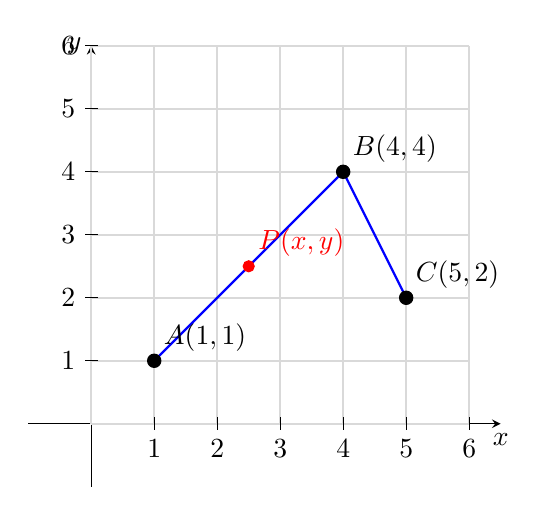
\begin{tikzpicture}[scale=0.8, >=stealth]
    % 绘制坐标轴
    \draw[->] (-1,0) -- (6.5,0) node[below] {$x$};
    \draw[->] (0,-1) -- (0,6) node[left] {$y$};
    \draw[thick, gray!30] (0,0) grid (6,6);
    
    % 标刻度
    \foreach \x in {1,...,6} \draw (\x,0.1) -- (\x,-0.1) node[below] {$\x$};
    \foreach \y in {1,...,6} \draw (0.1,\y) -- (-0.1,\y) node[left] {$\y$};
    
    % 绘制折线段 A-B-C
    \draw[thick, blue] (1,1) -- (4,4) -- (5,2);
    
    % 标注点
    \filldraw[black] (1,1) circle (3pt) node[above right] {$A(1,1)$};
    \filldraw[black] (4,4) circle (3pt) node[above right] {$B(4,4)$};
    \filldraw[black] (5,2) circle (3pt) node[above right] {$C(5,2)$};
    
    % 示意动点 P (例如取在 AB 上)
    \filldraw[red] (2.5,2.5) circle (2.5pt) node[above right] {$P(x,y)$};
    
    % 可选：标注折线
    %\node[blue] at (2.5,3) {折线段 $A-B-C$};
\end{tikzpicture}
\end{center}

(1) 当 \(a = -2\) 时，\(t\) 的最大值为 \_\_\_\_\_\_；

(2) 若 \(t\) 存在最大值，则 \(a\) 的取值范围为 \_\_\_\_\_\_。


（答案见第~\pageref{绝对值几何意义与坐标-题目1}~页）


\section{坐标轴-题目2}


在平面直角坐标系 \(xOy\) 中，对于点 \(A(x_1, y_1)\)，\(B(x_2, y_2)\)，令 \(m = x_1 + x_2\)，\(n = y_1 + y_2\)，将 \(|m - n|\) 称为点 \(A\) 与点 \(B\) 的特征值。对于图形 \(M\) 和图形 \(N\)，若点 \(A\) 为图形 \(M\) 上的任意一点，点 \(B\) 为图形 \(N\) 上的任意一点，且点 \(A\) 与点 \(B\) 的特征值存在最大值，则将该最大值称为图形 \(M\) 与图形 \(N\) 的特征值。

\begin{center}
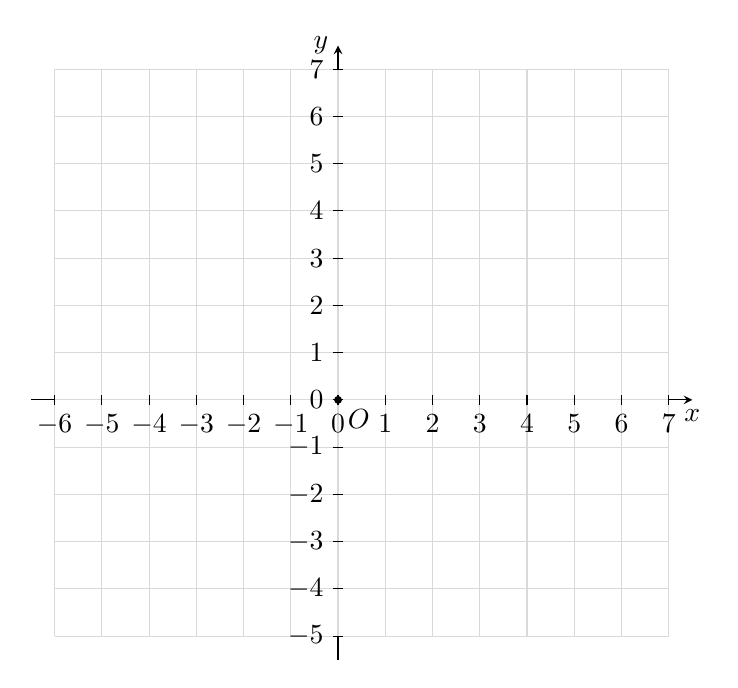
\begin{tikzpicture}[scale=0.6, >=stealth]
    % 坐标轴范围：x:-6~7, y:-5~7
    \draw[->] (-6.5,0) -- (7.5,0) node[below] {$x$};
    \draw[->] (0,-5.5) -- (0,7.5) node[left] {$y$};
    % 网格
    \draw[step=1, gray!30, thin] (-6,-5) grid (7,7);
    % 刻度
    \foreach \x in {-6,-5,...,7} \draw (\x,0.1) -- (\x,-0.1) node[below] {$\x$};
    \foreach \y in {-5,-4,...,7} \draw (0.1,\y) -- (-0.1,\y) node[left] {$\y$};
    % 原点
    \filldraw (0,0) circle (2pt) node[below right] {$O$};
\end{tikzpicture}
\end{center}

(1) 已知点 \(A(3,2)\)，\(B(2,-4)\)。

\begin{enumerate}
    \item[①] 点 \(A\) 与点 \(B\) 的特征值为 \_\_\_\_\_\_；
    \item[②] 已知点 \(C\) 在 \(y\) 轴上，若点 \(A\) 与点 \(C\) 的特征值为 \(5\)，则点 \(C\) 的坐标为 \_\_\_\_\_\_；
\end{enumerate}

(2) 已知点 \(D(6,0)\)，\(E(4,0)\)，将线段 \(DE\) 以每秒 \(1\) 个单位的速度向左平移，经过 \(t\ (t>0)\) 秒后得到线段 \(D_1E_1\)。

\begin{enumerate}
    \item[①] 已知点 \(F(2,4)\)，\(0 < t \le 8\)，求点 \(F\) 与线段 \(D_1E_1\) 的特征值 \(h\) 的取值范围；
    \item[②] 已知面积为 \(2\) 的正方形的对角线交点为 \(G(2t,2t)\)，且该正方形至少有一条边与坐标轴平行，记该正方形与线段 \(D_1E_1\) 的特征值为 \(k\)，则 \(k\) 的最小值为 \_\_\_\_\_\_；当 \(k \le 6\) 时，\(t\) 的取值范围为 \_\_\_\_\_\_。
\end{enumerate}


（答案见第~\pageref{坐标轴-题目2}~页）


\section{坐标轴-面积综合题目}

坐标轴和面积的关系：

\subsection{坐标轴-面积综合题目1}

\begin{center}

\includegraphics[width=1.0\textwidth]{坐标轴-动点-题目1.png}
\end{center}

（答案见第~\pageref{坐标轴-面积综合题目1}~页）



\section{已知面积求坐标轴-题目1 【难度：4星】}

如图，已知 \(A(0,a)\)，\(B(b,0)\)，且满足
\[
|a - 4| + \sqrt{b + 6} = 0
\]

% 插入图片
\begin{center}

\includegraphics[width=0.8\textwidth]{坐标轴-已知面积求坐标轴-题目1.png}
\end{center}

(1) 求 \(A\)、\(B\) 两点的坐标。

(2) 点 \(C(m,n)\) 在线段 \(AB\) 上，\(m\)、\(n\) 满足 \(n - m = 5\)，点 \(D\) 在 \(y\) 轴负半轴上，连 \(CD\) 交 \(x\) 轴的负半轴于点 \(M\)，且 \(S_{\triangle MBC} = S_{\triangle MOD}\)，求点 \(D\) 的坐标。

(3) 平移直线 \(AB\)，交 \(x\) 轴正半轴于 \(E\)，交 \(y\) 轴于 \(F\)，\(P\) 为直线 \(EF\) 上第三象限内的点，过 \(P\) 作 \(PG \perp x\) 轴于 \(G\)，若 \(S_{\triangle PAB} = 20\)，且 \(GE = 12\)，求点 \(P\) 的坐标。